%%%%%%%%%%%%%%%%%%%%%%%%%%%%%%%%%%%%%%%%%%%%%%%%%%%%%%%%%%
%% BEGIN PREAMBLE
\documentclass[10pt]{article}

\usepackage{hyperref}

\setlength{\parindent}{0pt}

%%%% Sets 1 inch margins on document
\usepackage[margin=1in]{geometry}

%%%% For math macros
\usepackage{amsmath}

%%%% Needed for including figures and other images
\usepackage{graphicx}

%%%% Adds ability to adjust document vertical spacing
% usage:
%   \setspace{1.5} % 1.5x for line spacing
\usepackage{setspace}

%%%% Needed for specifying the list items in enumerate env
% eg. (a,b,b) or (i,ii,iii), (1,2,3)
% usage:
%   \begin{enumerate} [label=(\alph*)] % for (a), (b), (c)
\usepackage{enumitem}

%%%% Defines Times New Roman as font
  % for math and text environments
\usepackage{newtxtext,newtxmath}

%%%% For H float option when inserting figure
%   [H] inserts figure _exactly_ where it is typeset
% usage:
%   begin{figure} [H]
\usepackage{float}

%%%% For fancy header and footer ;)
\usepackage{fancyhdr}
\pagestyle{fancy}
\fancyhead[LO,L]{Samuel Barton}
\fancyhead[CO,C]{ENGS31 - Homework 5}
\fancyhead[RO,R]{\today}
\fancyfoot[LO,L]{}
\fancyfoot[CO,C]{\thepage}
\fancyfoot[RO,R]{}
\renewcommand{\headrulewidth}{0.4pt}
\renewcommand{\footrulewidth}{0.4pt}

%%%% Setting margins in tabular environments
% For making equations (esp. fractions) fit in cells vertically
\usepackage{cellspace}
\cellspacetoplimit 4pt
\cellspacebottomlimit 4pt
%% END PREAMBLE %%
%%%%%%%%%%%%%%%%%%%%%%%%%%%%%%%%%%%%%%%%%%%%%%%%%%%%%%%%%%%%%%%

\begin{document}

\setstretch{1.25} % set spacing to 1.25x

% Assignment Name
\begin{centering}
  \section*{HOMEWORK 5}
\end{centering}

\subsection*{Question 1: White Noise Generator}

\subsubsection*{Part (a):}

\begin{figure} [H]
  \center
  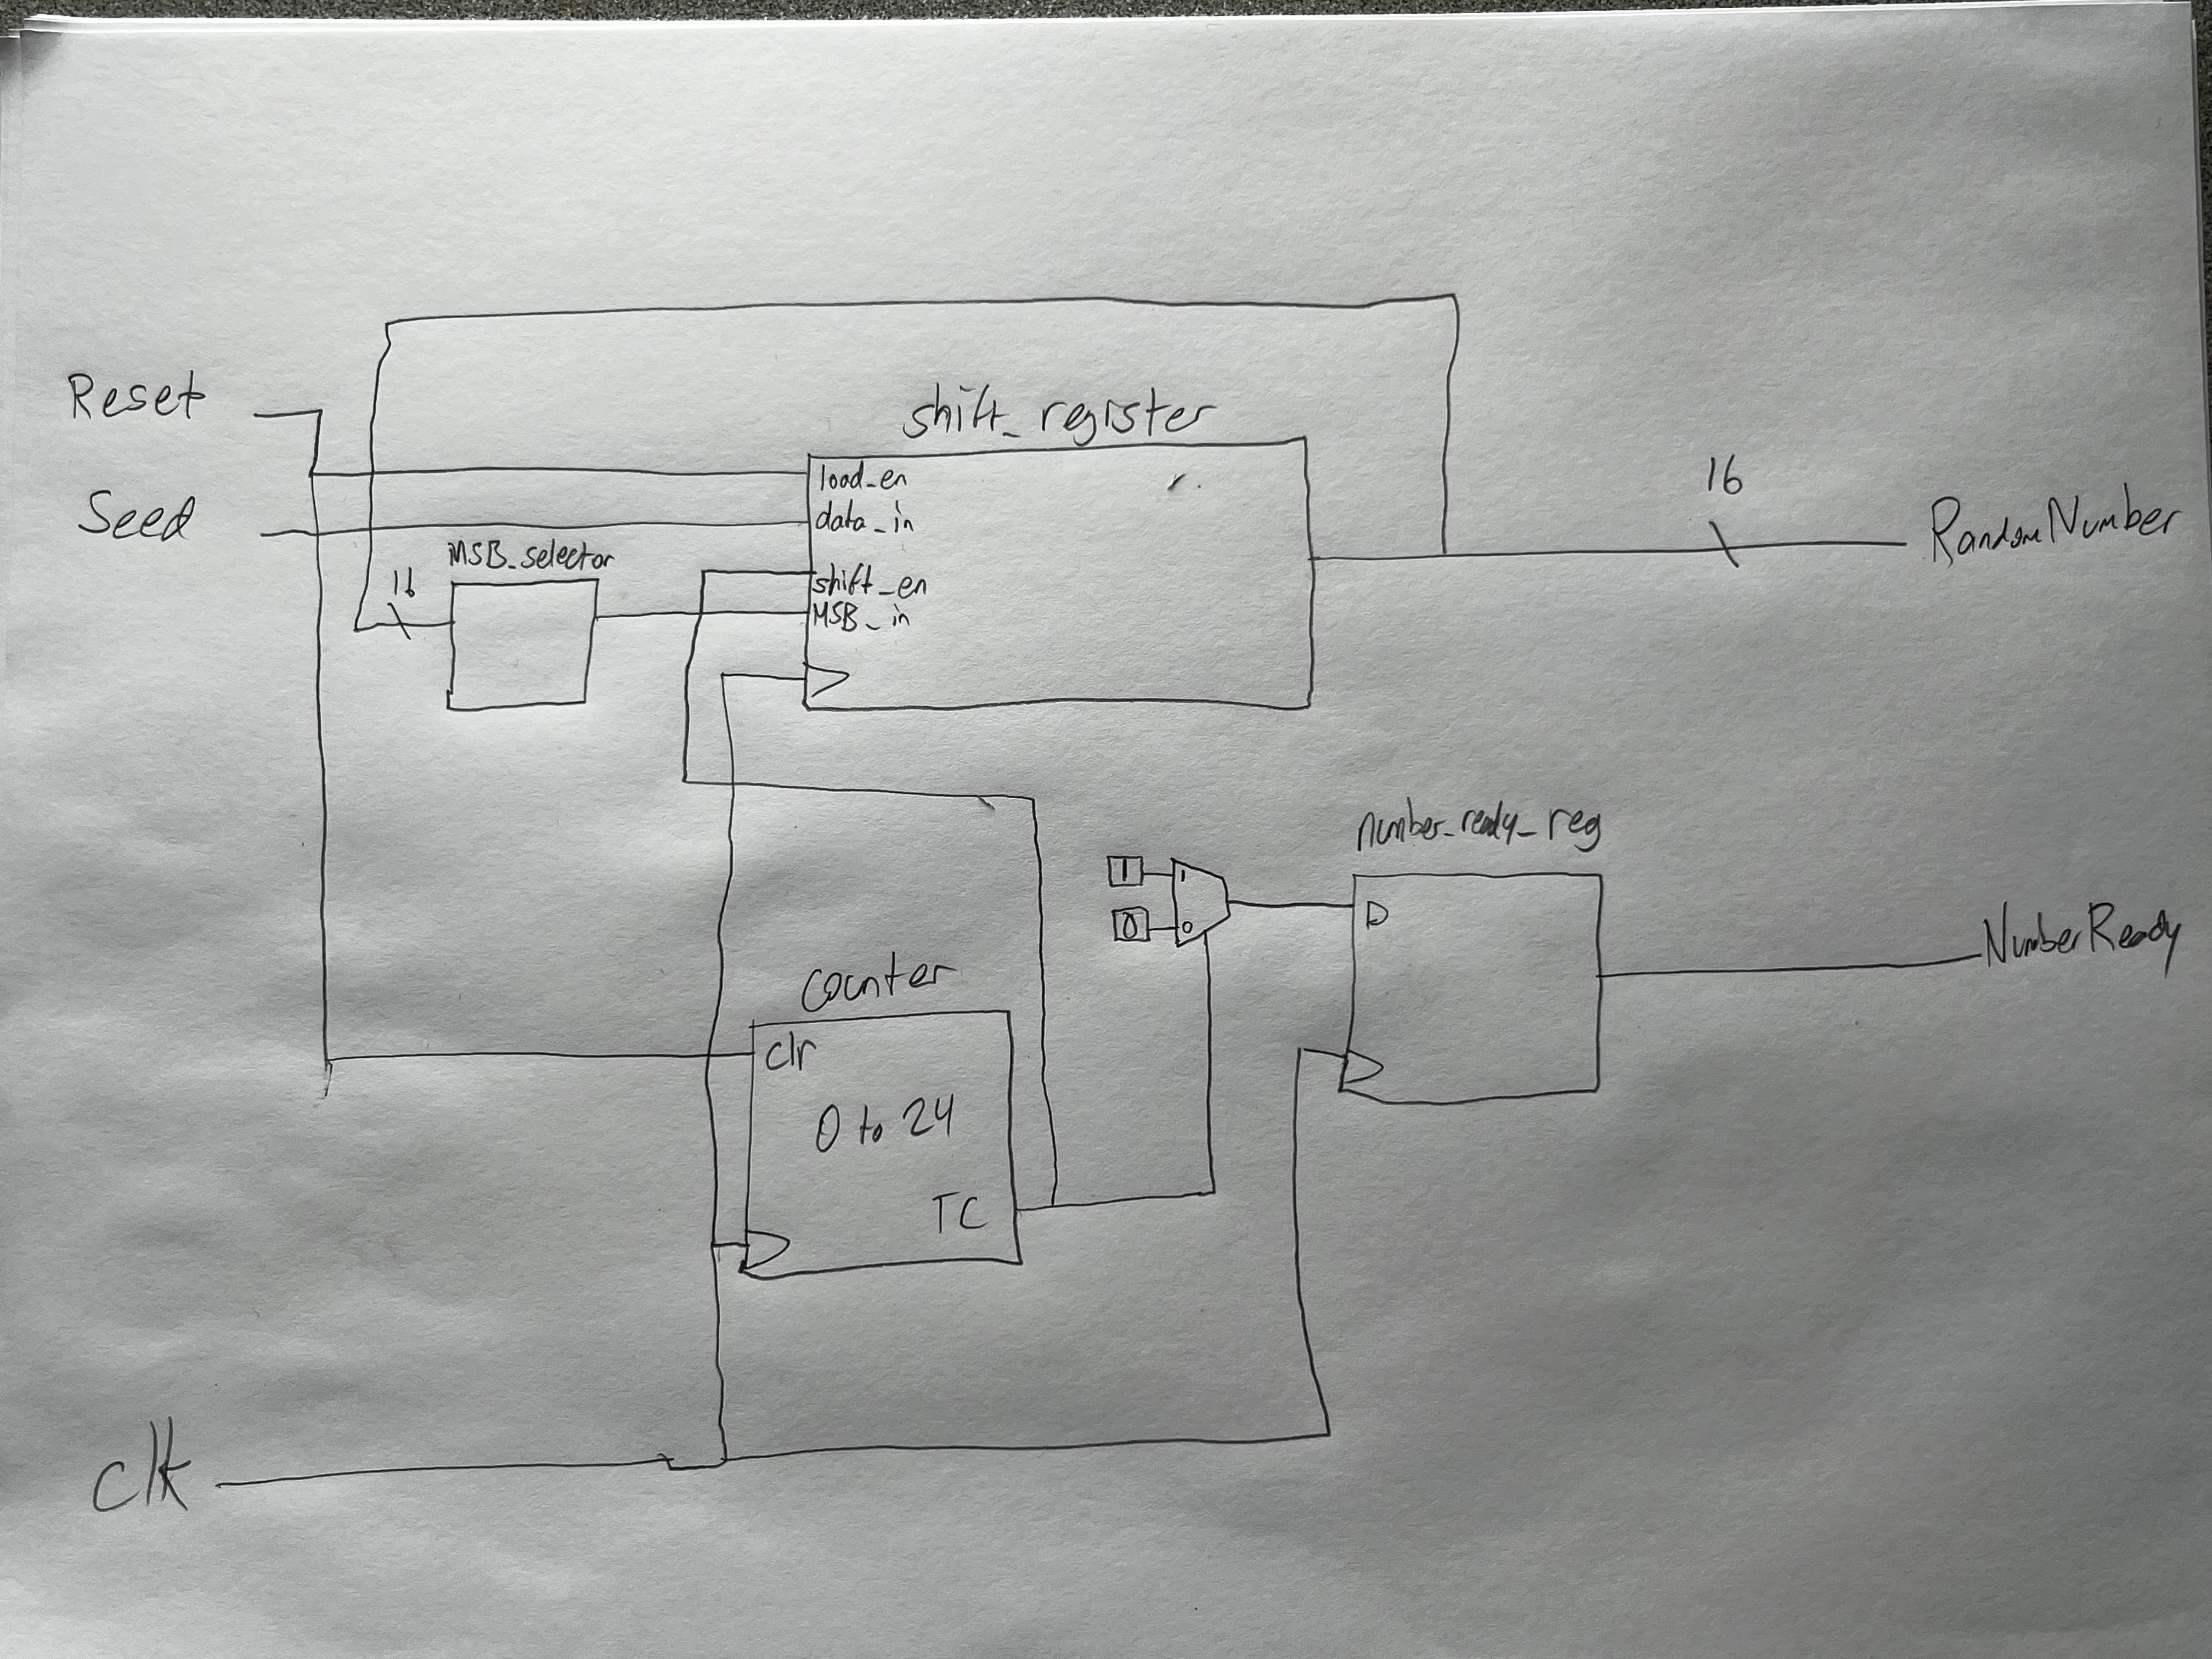
\includegraphics[width=0.75\textwidth]{figures/white_noise_bd.png}
  \caption{RTL-Level Block Diagram of the Fibonacci LFSR System}
\end{figure}

\subsubsection*{Part (b):}

EDA Playground link: \url{https://www.edaplayground.com/x/Qyzx}

\begin{figure} [H]
  \center
  \includegraphics[width=0.95\textwidth]{figures/white_noise_gen_tb.png}
  \caption{Waveform of Full Testbench for White Noise Generator, Annotated}
\end{figure}

\begin{figure} [H]
  \center
  \includegraphics[width=0.95\textwidth]{figures/zoomed_in_wng.png}
  \caption{Zoomed-in Waveform Showing 40 kHz Refresh Rate, Annotated}
\end{figure}

\subsection*{Question 2: Code Guessing Game}

\subsubsection*{Part (a):}

This system will require 8 four-bit registers, and 2 three-bit counters.

Four registers will be used to store the four numbers needed for storing the code, and the other four registers are needed for storing each guess for comparison.
The registers are chained together as with a shift register so that each entered number is first stored in the foremost register.
The enable pins of the registers will be high based on control signals from the controller and from the input pins.

For the two counters, one is for counting which number is being entered, and the other is for counting the number of guesses.
Both counters count up to 4, so 3 bits are needed.
When the counters reach their maximum count, a terminal count control signal is asserted to the controller, and the counter resets.

Other control signals: 

Inputs: EnteringCodeSignal(when player is entering code), EnteringGuessSignal(when player is entering guess), and CheckSignal(when the system checks the guess against the code). 

Outputs: NumberCountTC(When the player has entered the fourth code/guess number), GuessCountTC(When the player has guessed their fourth guess), and WinSignal(When the guess is equal to the code at the check state).

\subsubsection*{Part (b):}

\begin{figure} [H]
  \center
  \includegraphics[width=0.95\textwidth]{figures/datapath_image.png}
  \caption{Datapath}
\end{figure}

\subsubsection*{Part (c):}

\begin{figure} [H]
  \center
  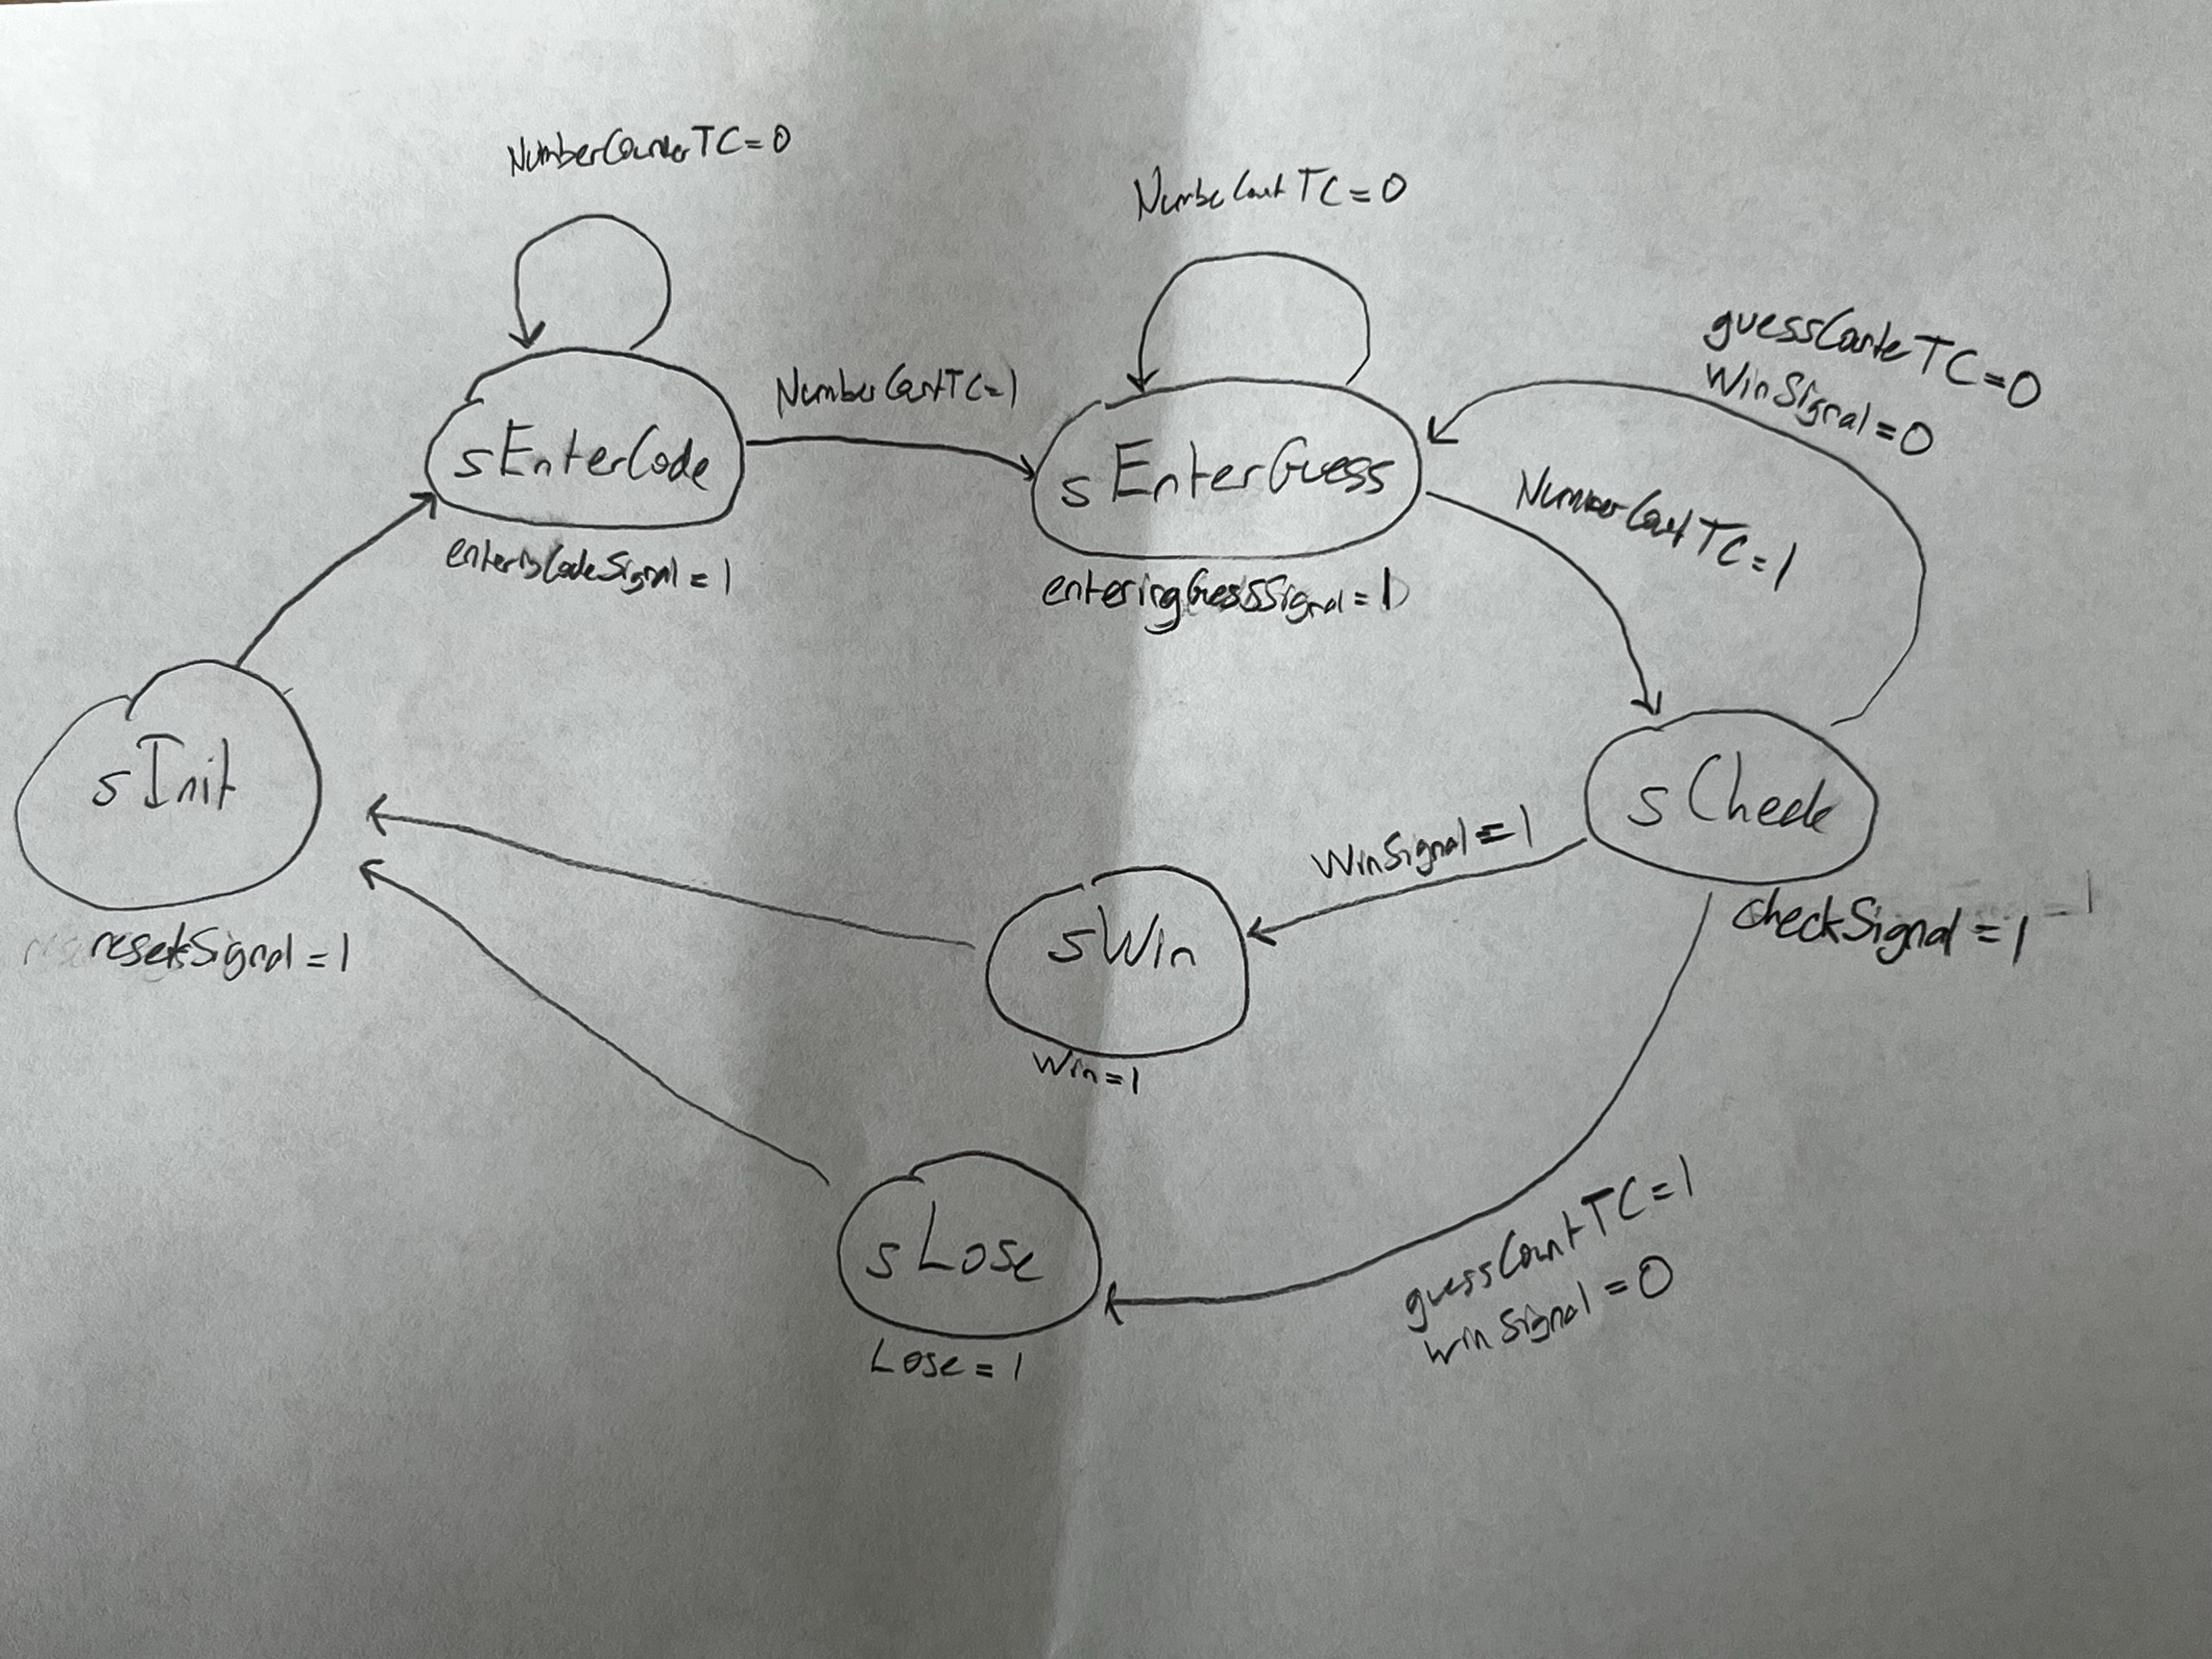
\includegraphics[width=0.95\textwidth]{figures/FSM.png}
  \caption{Finite State Machine}
\end{figure}

\subsubsection*{Part (d):}

EDA Playground link: \url{https://www.edaplayground.com/x/Qz5g}

\begin{figure} [H]
  \center
  \includegraphics[width=0.95\textwidth]{figures/game_operation.png}
  \caption{Full Game Operation, Annotated}
\end{figure}

\begin{figure} [H]
  \center
  \includegraphics[width=0.95\textwidth]{figures/guess.png}
  \caption{Zoomed-In Look at a Specific Guess, Annotated}
\end{figure}

\end{document}

